\documentclass[11pt,a4paper]{report}
\usepackage[spanish,es-nodecimaldot]{babel}	% Utilizar español
\usepackage[utf8]{inputenc}					% Caracteres UTF-8
\usepackage{graphicx}						% Imagenes
\usepackage[hidelinks]{hyperref}			% Poner enlaces sin marcarlos en rojo
\usepackage{fancyhdr}						% Modificar encabezados y pies de pagina
\usepackage{float}							% Insertar figuras
\usepackage[textwidth=390pt]{geometry}		% Anchura de la pagina
\usepackage[nottoc]{tocbibind}				% Referencias (no incluir num pagina indice en Indice)
\usepackage{enumitem}						% Permitir enumerate con distintos simbolos
\usepackage[T1]{fontenc}					% Usar textsc en sections
\usepackage{amsmath}						% Símbolos matemáticos
\usepackage{listings}
\usepackage{longtable}

% Comando para poner el nombre de la asignatura
\newcommand{\asignatura}{Simulación de Sistemas}
\newcommand{\autor}{Vladislav Nikolov Vasilev}
\newcommand{\titulo}{PRÁCTICA 1}
\newcommand{\subtitulo}{Diferentes Modelos de Simulación}

% Configuracion de encabezados y pies de pagina
\pagestyle{fancy}
\lhead{\autor{}}
\rhead{\asignatura{}}
\lfoot{Grado en Ingeniería Informática}
\cfoot{}
\rfoot{\thepage}
\renewcommand{\headrulewidth}{0.4pt}		% Linea cabeza de pagina
\renewcommand{\footrulewidth}{0.4pt}		% Linea pie de pagina

\begin{document}
\pagenumbering{gobble}

% Pagina de titulo
\begin{titlepage}

\begin{minipage}{\textwidth}

\centering


\includegraphics[scale=0.5]{img/ugr.png}\\

\textsc{\Large \asignatura{}\\[0.2cm]}
\textsc{GRADO EN INGENIERÍA INFORMÁTICA}\\[1cm]

\noindent\rule[-1ex]{\textwidth}{1pt}\\[1.5ex]
\textsc{{\Huge \titulo\\[0.5ex]}}
\textsc{{\Large \subtitulo\\}}
\noindent\rule[-1ex]{\textwidth}{2pt}\\[3.5ex]

\end{minipage}

\vspace{0.5cm}

\begin{minipage}{\textwidth}

\centering

\textbf{Autor}\\ {\autor{}}\\[2.5ex]
\textbf{Rama}\\ {Computación y Sistemas Inteligentes}\\[2.5ex]
\vspace{0.3cm}


\includegraphics[scale=0.3]{img/etsiit.jpeg}

\vspace{0.7cm}
\textsc{Escuela Técnica Superior de Ingenierías Informática y de Telecomunicación}\\
\vspace{1cm}
\textsc{Curso 2018-2019}
\end{minipage}
\end{titlepage}

\pagenumbering{arabic}
\tableofcontents
\thispagestyle{empty}				% No usar estilo en la pagina de indice

\newpage

\setlength{\parskip}{1em}

\chapter{Mi primer modelo de Montecarlo}

\section{Pruebas iniciales con el modelo}

Inicialmente, se ha probado el modelo para ver cómo funcionaba. Se ha ejecutado el modelo una serie de
veces (10 para ser más precisos), y se han almacenado los resultados. Estos resultados pueden verse a
continuación:

\begin{table}[H]
\centering
\begin{tabular}{c|c}
\textbf{Mejor posición inicial ($c$)} & \textbf{Mejor distancia} \\ \hline
95                              & 6.525780                 \\
94                              & 6.472190                 \\
94                              & 6.513340                 \\
94                              & 6.531020                 \\
94                              & 6.498630                 \\
93                              & 6.512340                 \\
94                              & 6.469870                 \\
94                              & 6.487920                 \\
94                              & 6.486590                 \\
94                              & 6.478660                
\end{tabular}
\caption{Resultados de mejor posición inicial y mejor distancia para 10 ejecuciones.}
\label{aparc-tabla}
\end{table}

Como se puede apreciar, parece que hay cierta semejanza entre los resultados obtenidos en cada
ejecución. Se puede ver que el valor de $c$ obtenido es muy similar en casi todos los casos, siendo
la moda $c = 94$, y la media un valor muy próximo a éste. Los valores de la mejor distancia también
son muy próximos entre sí, ya que todos ellos rondan, aproximadamente, las 6.5 plazas. Por tanto, el
modelo es capaz de producir unos resultados muy similares a pesar de que utiliza cierta ``aleatoriedad''.

Si estudiamos cómo evoluciona el valor de la distancia al destino a medida que cambia el valor de $c$, nos
encontramos con la siguiente gráfica:

\begin{figure}[H]
\centering
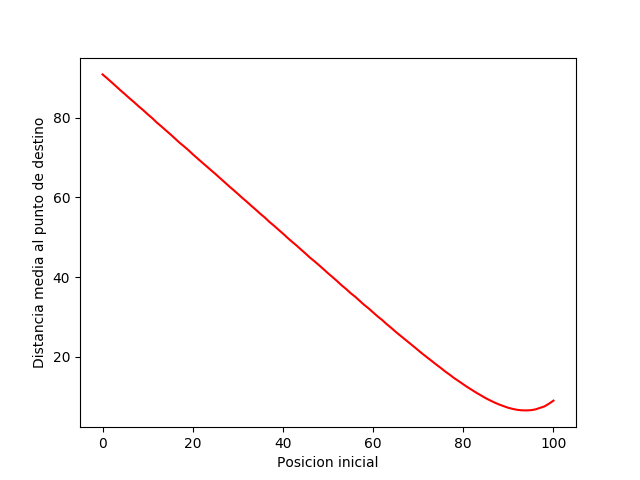
\includegraphics[scale=0.6]{img/c-dist.png}
\caption{Evolución del valor de la distancia al destino en función del valor de la posición inicial.}
\label{aparc-grafica}
\end{figure}

Como se puede ver, existe una tendencia a que, cuanto más cerca de la posición a la que se quiera llegar
se comienza a buscar sitio (es decir, cuanto más alto sea el valor de $c$), menor será la distancia hasta
el destino. Esto es completamente lógico, ya que al comenzar a buscar sitio a partir de una posición
muy lejana al destino, mayor será la distancia hasta éste en caso de que se encuentre una plaza libre. Teniendo
en cuenta que se escoge la primera plaza libre, ésta puede quedar muy lejos del destino, que es lo que se puede
apreciar en la gráfica.

El valor ideal de $c$, con las condiciones en las que estamos, parece ser $c = 94$. A partir de ahí, se puede ver
que existe un ligero incremento en la distancia al destino, posiblemente porque se aparque más lejos debido a que
no se encuentre una plaza libre en posiciones más cercanas al destino.

Por tanto, a vista de los resultados que hemos obtenido, podemos afirmar con bastante certeza que la plaza ideal
a partir de la que empezar sitio para aparcar es aproximadamente la 94.

\section{Experimentación con los parámetros}

Se han realizado una serie de experimentaciones con los parámetros con los que se puede llamar al programa.
A continuación, se muestran algunos de los resultados obtenidos.

\subsection{Modificación de la posición destino}

Se ha probado a modificar la posición destino, estableciendo que $x = 150$, y se han realizado 10 ejecuciones.
A continuación, se pueden ver los resultados obtenidos:

\begin{table}[H]
\centering
\begin{tabular}{c|c}
\textbf{Mejor posición inicial ($c$)} & \textbf{Mejor distancia} \\ \hline
144                              & 6.438900                 \\
144                              & 6.438900                 \\
144                              & 6.438900                 \\
143                              & 6.472200                 \\
143                              & 6.472200                 \\
143                              & 6.472200                 \\
143                              & 6.472200                 \\
143                              & 6.472200                 \\
143                              & 6.472200                 \\
143                              & 6.358800                
\end{tabular}
\caption{Resultados de mejor posición inicial y mejor distancia para 10 ejecuciones con
con posición destino $x = 150$.}
\label{aparc-150-tabla}
\end{table}

\begin{figure}[H]
\centering
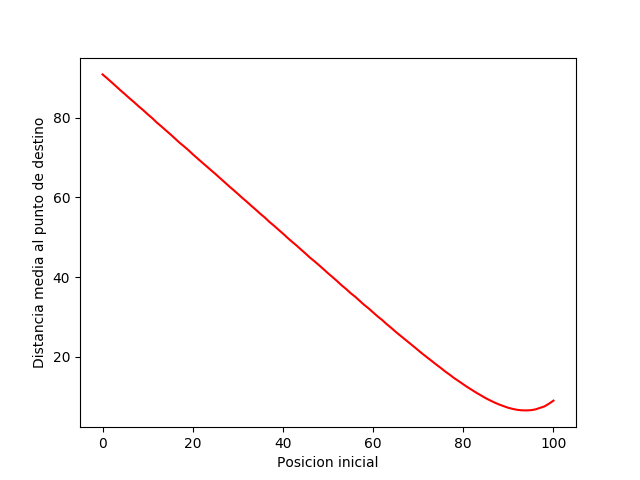
\includegraphics[scale=0.47]{img/c-dist.png}
\caption{Evolución del valor de la distancia al destino en función del valor de la posición inicial para $x = 150$.}
\label{aparc-150-grafica}
\end{figure}

Los resultados obtenidos en la tabla \ref{aparc-150-tabla} son muy parecidos a los que obtuvimos en \ref{aparc-tabla},
solo que los valores de $c$ han cambiado, aunque siguen unos patrones parecisos. En este caso, la moda parece ser 143,
y la media tiende a ese valor. Las mejores distancias están también muy próximas, y no se ve mucha disparidad.

Además, tal y como se hizo en el caso anterior, se ha obtenido una gráfica que muestra la evolución de la distancia media
en función del valor de $c$, la cuál se puede ver en la figura \ref{aparc-150-grafica}. Como se puede observar, sigue
un patrón muy parecido al que se puede ver en la figura \ref{aparc-grafica}, así que parece que no es un parámetro
que influya demasiado por sí solo.

\subsection{Modificación de la probabilidad de ocupación}

Se ha probado a variar la probabilidad de ocupación para ver cómo es afectada la salida. A continuación, se pueden ver
los resultados que se han obtenido tras realizar 11 ejecuciones:

\begin{table}[H]
\begin{tabular}{c|c|c}
\textbf{Probabilidad de ocupación} & \textbf{Mejor posición inicial ($c$)} & \textbf{Mejor distancia} \\ \hline
0.01                               & 99                              & 0.008400                 \\
0.1                                & 99                              & 0.100000                 \\
0.2                                & 99                              & 0.213100                 \\
0.3                                & 99                              & 0.344800                 \\
0.4                                & 99                              & 0.495100                 \\
0.5                                & 98                              & 0.744800                 \\
0.6                                & 98                              & 1.074900                 \\
0.7                                & 98                              & 1.659600                 \\
0.8                                & 97                              & 2.901000                 \\
0.9                                & 94                              & 6.477300                 \\
0.99                               & 36                              & 67.957802               
\end{tabular}
\caption{Valores de la mejor posición inicial y distancia en función de la probabilidad de ocupación.}
\label{aparc-tabla-prob}
\end{table}

Es interesante ver cómo, a medida que va incrementando la probabilidad de ocupación, los valores de $c$ y de distancia
van cambiando, y se van haciendo cada vez peores. Se puede ver como el valor de $c$ va disminuyendo a medida que va aumentando
la probabilidad, lo cuál afecta directamente a la distancia, aumentándola proporcionalmente cada vez que disminuye el valor de
$c$. Todo esto se debe a que, cuanto menor sea la probabilidad de ocupación, más cerca del destino se podrá encontrar un sitio.
Todo esto se puede ver gráficamente en la siguiente figura:

\begin{figure}[H]
\centering
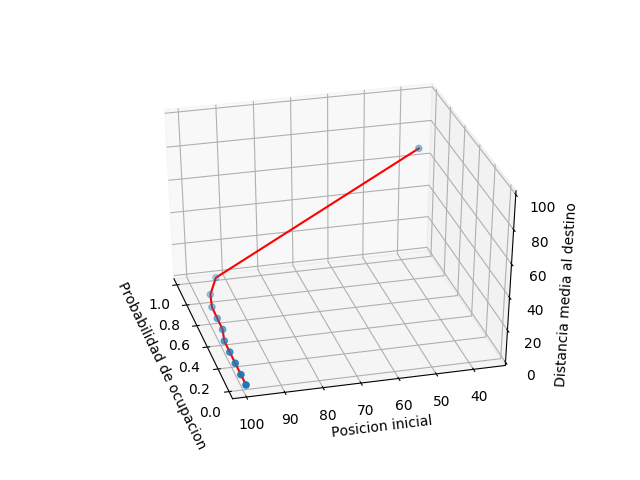
\includegraphics[scale=0.6]{img/aparc-prob-3d.png}
\caption{Representación 3D de la distancia media al destino en función de la probabilidad de ocupación y
la posición inicial.}
\label{aparc-3d-prob}
\end{figure}

Si se prueba con valores muy extremos, como por ejemplo con probabilidad de ocupación de 0.999, se obtiene el
siguiente error:

\begin{figure}[H]
\centering
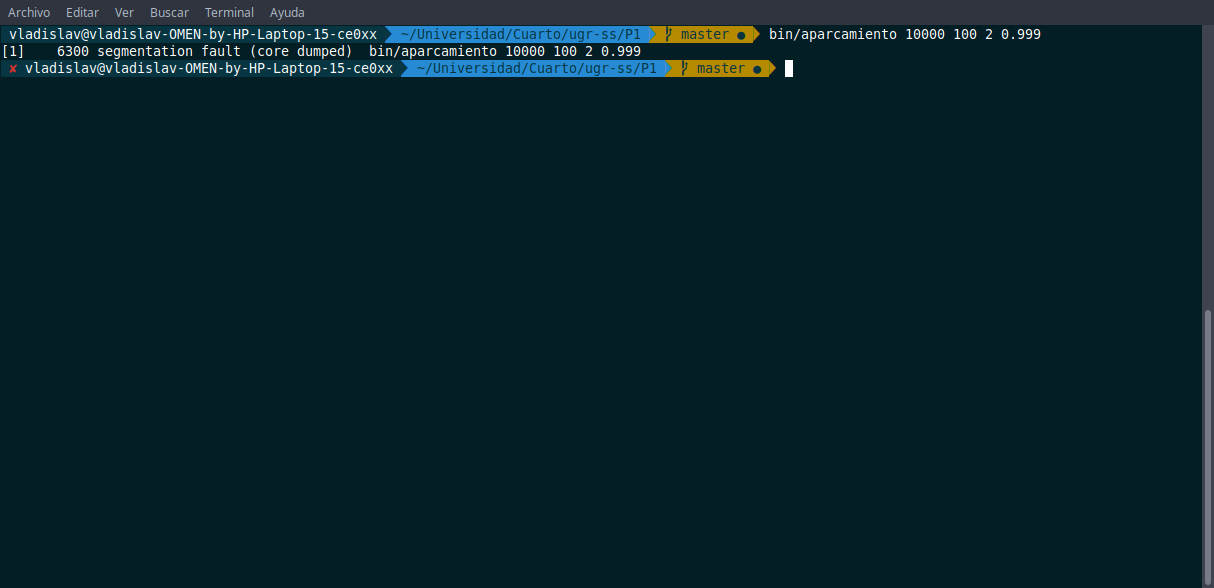
\includegraphics[scale=0.3]{img/aparc-prob-error.png}
\caption{Error al ejecutar el programa \textit{aparcamiento} con 0.999 de probabilidad de ocupación.}
\end{figure}

Esto se debe a que no se consigue encontrar sitio libre y se supera el tamaño del vector que representa las posiciones,
lo cuál genera un fallo de segmentación al intentar acceder a posiciones no válidas de memoria.

\subsection{Modificación del nivel de visión}

Vamos a intentar variar ahora el nivel de visión para ver cómo son afectados los resultados. Estos son los resultados
obtenidos tras haber realizado 11 ejecuciones:

\begin{table}[H]
\begin{tabular}{c|c|c}
\textbf{Alcance de visión} & \textbf{Mejor posición inicial ($c$)} & \textbf{Mejor distancia} \\ \hline
2                          & 94                              & 6.480800                 \\
4                          & 94                              & 6.339700                 \\
6                          & 94                              & 6.069100                 \\
8                          & 93                              & 5.706100                 \\
10                         & 92                              & 5.505300                 \\
15                         & 90                              & 5.244000                 \\
20                         & 86                              & 4.954400                 \\
25                         & 83                              & 4.890900                 \\
30                         & 82                              & 4.778700                 \\
50                         & 72                              & 4.687100                 \\
100                        & 80                              & 4.624000                
\end{tabular}
\caption{Valores de la mejor posición inicial y distancia en función del alcance de visión.}
\label{aparc-tabla-vis}
\end{table}

Como se puede ver, aquí también al aumentar el valor del alcance de visión, el valor de $c$ disminuye. Sin embargo,
a diferencia del caso anterior, la mejor distancia media va disminuyendo, posiblemente debido a que se tenga más
conocimiento de las posiciones venideras. En el caso extremo en el que se ven todas las plazas de aparcamiento,
se ve que la distancia media es la mínima. Todo esto se puede ver en la siguiente figura:

\begin{figure}[H]
\centering
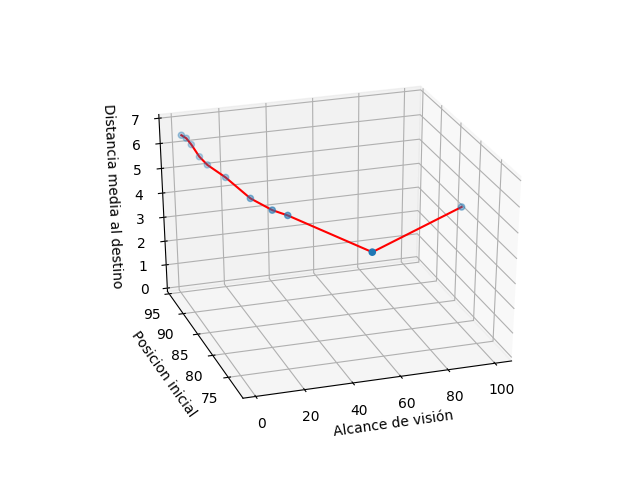
\includegraphics[scale=0.49]{img/aparc-vis-3d.png}
\caption{Representación 3D de la distancia media al destino en función del alcance de visión y
la posición inicial.}
\label{aparc-3d-vis}
\end{figure}

\subsection{Modificación de la visión y la probabilidad de ocupación}

En este último apartado, se ha querido ver qué pasa si se modifican dos variables a la vez. Para ello, se van a
modificar tanto el alcance de visión como la probabilidad de ocupación.

Los resultados de haber probado 9 combinaciones de parámetros se pueden ver en la siguiente tabla:

\begin{table}[H]
\resizebox{\columnwidth}{!}{%
\begin{tabular}{c|c|c|c}
\textbf{\begin{tabular}[c]{@{}c@{}}Probabilidad\\ de ocupación\end{tabular}} & \textbf{Alcance de visión} & \textbf{Mejor posición inicial  ($c$)} & \textbf{Mejor distancia} \\ \hline
0.4                                                                          & 5                          & 98                              & 0.480700                 \\
0.4                                                                          & 10                         & 94                              & 0.469800                 \\
0.4                                                                          & 15                         & 90                              & 0.459100                 \\
0.5                                                                          & 5                          & 97                              & 0.660100                 \\
0.5                                                                          & 10                         & 96                              & 0.661500                 \\
0.5                                                                          & 15                         & 90                              & 0.655300                 \\
0.6                                                                          & 5                          & 96                              & 1.472600                 \\
0.6                                                                          & 10                         & 95                              & 1.362600                 \\
0.6                                                                          & 15                         & 91                              & 1.364300                
\end{tabular}
}%
\caption{Valores de la mejor posición inicial y distancia en función de la probabilidad de ocupación y el alcance
de visión.}
\label{aparc-tabla-prob-vis}
\end{table}

Como se puede ver, aún con la misma probabilidad de ocupación, el hecho de tener un mayor alcance de visión permite
disminuir la mejor distancia media al destino, lo cuál sugiere que las suposiciones anteriores sobre que el alcance de
visión permite tener más conocimiento sobre el problema son correctas. También se puede ver un claro patrón en el que,
si se incrementa solo la probabilidad de ocupación sin cambiar el alcance de visión, la mejor distancia media empeora,
pero al incrementar el alcance, ésta disminuye, tal y como se puede observar en las tablas \ref{aparc-tabla-prob} y
\ref{aparc-tabla-vis}.

\newpage

\chapter{Mi primer modelo de simulación discreto}

\section{Estudio experimental del número de repuestos}

Se va a realizar un estudio experimental del número de repuestos mínimo que se necesita. Para ello, se va a ejecutar
el programa una serie de veces, con un número de piezas de repuesto y de repeticiones diferente. En concreto, se van
a probar 5, 7, 9, 11 y 12 piezas, y 1, 10, 100, 500 y 1000 repeticiones. A continuación se pueden ver los resultados:

\begin{longtable}{c|c|c}
\textbf{\begin{tabular}[c]{@{}c@{}}Nº piezas\\ de repuesto\end{tabular}} & \textbf{Nº de repeticiones} & \textbf{\begin{tabular}[c]{@{}c@{}}Media del \% de\\ tiempo de desprotección\end{tabular}} \\ \hline
5                                                                        & 1                           & 37.1069                                                                                    \\
7                                                                        & 1                           & 11.7863                                                                                    \\
9                                                                        & 1                           & 3.26835                                                                                    \\
11                                                                       & 1                           & 0.554182                                                                                   \\
12                                                                       & 1                           & 0                                                                                          \\ \hline
5                                                                        & 10                          & 31.9152                                                                                    \\
7                                                                        & 10                          & 14.5627                                                                                    \\
9                                                                        & 10                          & 2.8476                                                                                     \\
11                                                                       & 10                          & 0.944855                                                                                   \\
12                                                                       & 10                          & 0.410312                                                                                   \\ \hline
5                                                                        & 100                         & 38.0701                                                                                    \\
7                                                                        & 100                         & 16.1558                                                                                    \\
9                                                                        & 100                         & 4.23885                                                                                    \\
11                                                                       & 100                         & 1.10964                                                                                    \\
12                                                                       & 100                         & 0.593476                                                                                   \\ \hline
5                                                                        & 500                         & 36.92                                                                                      \\
7                                                                        & 500                         & 15.3941                                                                                    \\
9                                                                        & 500                         & 4.94555                                                                                    \\
11                                                                       & 500                         & 1.05448                                                                                    \\
12                                                                       & 500                         & 0.394317                                                                                   \\ \hline
5                                                                        & 1000                        & 37.2712                                                                                    \\
7                                                                        & 1000                        & 15.5255                                                                                    \\
9                                                                        & 1000                        & 4.83779                                                                                    \\
11                                                                       & 1000                        & 0.943597                                                                                   \\
12                                                                       & 1000                        & 0.435409       
\end{longtable}

Si analizamos los resultados detenidamente, podemos ver que, al aumentar el número de repeticiones, los resultados
toman unos valores que se acercan más al comportamiento promedio. Esto se debe a que en el modelo existen ciertas
variables aleatorias. Por tanto, sacar conclusiones a partir de una única ejecución no sería algo válido. Habría
que hacer un gran número de repeticiones (como por ejemplo 500, 1000 o más) para sacar conclusiones verdaderamente válidas.

Teniendo en cuenta lo dicho anteriormente y a la vista de todos los resultados que se han obtenido,
se puede concluir que el número mínimo de piezas de repuesto que se necesitaría para que el
tiempo de desprotección total sea inferior al 1\% son \textbf{12 piezas}. Podemos concluir esto porque, viendo
los resultados que se han obtenido al variar el número de repeticiones, en el caso de 12 piezas nunca se pasa de ese
umbral. El hecho de tener 11 piezas es suficiente en algunos casos, pero en otros, se supera ese porcentaje de tiempo.
Por tanto, aunque podríamos decir que el valor óptimo de piezas de repuesto está entre 11 y 12, vamos a quedarnos con
las 12, tal y cómo hemos dicho anteriormente, debido a que ofrece más ``seguridad'' tener una pieza más.

\section{Experimentación con los parámetros}

Habiendo determinado el número mínimo de componentes de repuesto necesarios, vamos a ver cómo modificando los valores
de algunos de los parámetros cambian los resultados obtenidos.

\subsection{Modificación del tiempo de reparación}

Vamos a disminuir el tiempo de reparación para ver cuál sería en este caso el mínimo número de componentes que
necesitaríamos. Para ello, vamos a cambiar los tiempos para que se tarde entre 5 y 15 días, siguiendo una distribución
uniforme. Para evitar tener tantos datos como antes, vamos a considerar solo 100, 500 y 1000 repeticiones, ya que
hemos visto que son una buena aproximación porque se trata de un resultado medio.

A continuación se pueden ver los resultados:

\begin{table}[H]
\begin{tabular}{c|c|c}
\textbf{\begin{tabular}[c]{@{}c@{}}Nº piezas\\ de repuesto\end{tabular}} & \textbf{Nº de repeticiones} & \textbf{\begin{tabular}[c]{@{}c@{}}Media del \% de\\ tiempo de desprotección\end{tabular}} \\ \hline
5                                                                        & 100                         & 3.74915                                                                                    \\
7                                                                        & 100                         & 0.412021                                                                                   \\
9                                                                        & 100                         & 0.0101209                                                                                  \\
11                                                                       & 100                         & 0                                                                                          \\
12                                                                       & 100                         & 0                                                                                          \\ \hline
5                                                                        & 500                         & 3.7748                                                                                     \\
7                                                                        & 500                         & 0.354648                                                                                   \\
9                                                                        & 500                         & 0.026469                                                                                   \\
11                                                                       & 500                         & 0.000546791                                                                                \\
12                                                                       & 500                         & 0                                                                                          \\ \hline
5                                                                        & 1000                        & 3.56635                                                                                    \\
7                                                                        & 1000                        & 0.393049                                                                                   \\
9                                                                        & 1000                        & 0.02624                                                                                    \\
11                                                                       & 1000                        & 0.000315176                                                                                \\
12                                                                       & 1000                        & 0.000970965                                                                               
\end{tabular}
\end{table}

Como se puede ver claramente, parece ser que con un número de 6-7 piezas de repuesto se puede conseguir que el porcentaje
del tiempo de desprotección sea inferior al 1\%. Este número es inferior al que teníamos antes, el cuál rondaba las 12 piezas,
lo cuál es bastante bueno, ya que implica invertir menos en piezas, pero por otra parte, implica invertir más en las reparaciones.
Si estas no son muy caras (y teniendo en cuenta que las piezas de por sí son caras), sería más recomendable buscar
una reparación más rápida que disponer de un número mayor de piezas.

\subsection{Modificación del tiempo de vida}

Vamos a aumentar el tiempo de vida de los componentes hasta 50 días de media, siguiendo una distribución exponencial, para
ver como esta modificación afecta a la cantidad mínima de componentes de repuesto que se necesitarían. Para ello, se ha
seguido un proceso similar al que se ha llevado a cabo en la sección anterior.

A continuación se pueden ver los resultados que se han obtenido:

\begin{table}[H]
\begin{tabular}{c|c|c}
\textbf{\begin{tabular}[c]{@{}c@{}}Nº piezas\\ de repuesto\end{tabular}} & \textbf{Nº de repeticiones} & \textbf{\begin{tabular}[c]{@{}c@{}}Media del \% de\\ tiempo de desprotección\end{tabular}} \\ \hline
5                                                                        & 100                         & 2.6056                                                                                     \\
7                                                                        & 100                         & 0.163214                                                                                   \\
9                                                                        & 100                         & 0.0138627                                                                                  \\
11                                                                       & 100                         & 0                                                                                          \\
12                                                                       & 100                         & 0                                                                                          \\ \hline
5                                                                        & 500                         & 2.34215                                                                                    \\
7                                                                        & 500                         & 0.163914                                                                                   \\
9                                                                        & 500                         & 0.0128837                                                                                  \\
11                                                                       & 500                         & 0                                                                                          \\
12                                                                       & 500                         & 0                                                                                          \\ \hline
5                                                                        & 1000                        & 2.4367                                                                                     \\
7                                                                        & 1000                        & 0.207335                                                                                   \\
9                                                                        & 1000                        & 0.0154164                                                                                  \\
11                                                                       & 1000                        & 0                                                                                          \\
12                                                                       & 1000                        & 0                                                                                         
\end{tabular}
\end{table}

En este caso, con esta modificación, se obtienen unos resultados muy parecidos al caso anterior, ya que parece que el
número mínimo de componentes de repuesto ronda las 6-7 piezas. No obstante, aunque los resultados sean similares, parece
que el porcentaje del tiempo de desprotección es menor en este caso, lo cuál parece indicar que tener componentes más
duraderos es mejor que tener unos tiempos de reparación más pequeños. En la siguiente gráfica, se pueden ver
las diferencias:

\begin{figure}[H]
\centering
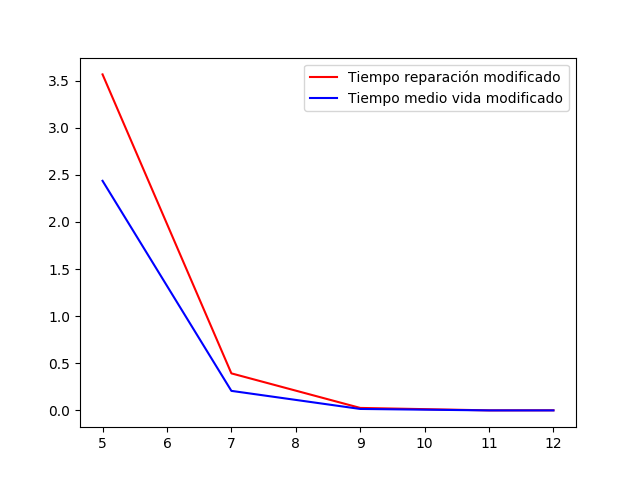
\includegraphics[scale=0.55]{img/radar.png}
\caption{Gráfica comparativa para 1000 repeticiones modificando el tiempo de reparación y el tiempo medio de vida.}
\end{figure}

Como se puede ver, existe cierta diferencia, aunque a medida que se van aumentando el número de piezas, ésta se hace
menos notable. Esta diferencia puede deberse a que el valor escogido como tiempo medio de vida sea bastante más alto que
los valores que se habían escogido como extremos del intervalo del tiempo de reparación; es decir, que se ha variado más
el tiempo medio de vida que el de reparación. Pero, parece que en este caso, si tuvieramos que escoger alguna de las
dos opciones sin considerar nada más, parece que sería más recomendable escoger piezas con una mayor duración, ya que
ofrecen una mayor protección.

\subsection{Conclusión}

Parece que tener unos tiempos de reparación más bajos y disponer de componentes más duraderos permite reducir el número
de componentes de repuesto necesarios. Parece que estos dos parámetros tienen bastante influencia en este número, así que,
en caso de querer determinar cuántos componentes necesitaríamos como mínimo, tenemos que considerar, además del precio de
éstos, cuánto tiempo se tardaría en reparar y el tiempo de vida medio de éstos. Dependiendo de cuáles sean los valores
de estos tiempos, nos interesará tener un mayor o un menor número de componentes.

También hay que considerear que, al ser los procesos de reparación más rápidos, éstos pueden ser más caros. Lo mismo pasa
con los componentes de mayor durabilidad: sus precios pueden ser mayores que unos que duran bastante menos tiempo. Por tanto,
en una situación real, también tenemos que tener en cuenta el factor económico para tomar una decisión con los datos que
nos ofrece la simulación, ya que estos factores no se han tenido en cuenta a la hora de desarrollar el modelo.

\newpage

\chapter{Mi primer modelo de simulación continuo}


\end{document}

